\documentclass[12pt, a4paper]{article}
\usepackage[utf8]{inputenc}
\usepackage[T1]{fontenc}
\usepackage[french]{babel}
\usepackage{amsmath, amssymb, amsfonts}
\usepackage{graphicx}
\usepackage{geometry}
\usepackage{hyperref}
\usepackage{float}

\geometry{margin=2.5cm}

\title{Maillages et simulation de la pollution acoustique}
\author{Yann MOUSSU}

\begin{document}

\maketitle

\tableofcontents
\newpage

\section{Introduction}
Ce rapport présente l'implémentation numérique complète d'un solveur pour l'équation de Helmholtz, visant à étudier la pollution acoustique et la dispersion numérique. Le projet est divisé en deux parties : la première est consacrée à la structure, l'optimisation et la qualité des maillages (réguliers et déformés) ; la seconde porte sur l'analyse approfondie de la précision et de la dispersion de la méthode des éléments finis (FEM).

\section{Structure et qualité du maillage}

\subsection{Structure de données et optimisation}
Pour optimiser les calculs, nous avons adopté une structure de données dites \textit{aplaties} (flat). Le maillage est représenté par les tableaux NumPy \texttt{node\_coords}, \texttt{elem2nodes} et \texttt{p\_elem2nodes}. 
Afin de garantir des performances optimales sur des maillages denses, les calculs géométriques primaires ont été \textbf{vectorisés} (ex: calcul simultané des aires par produit vectoriel matriciel).

\subsection{Outils géométriques avancés et extraction de frontière}
L'implémentation intègre le calcul exact du barycentre par élément ainsi qu'un algorithme de subdivision automatique pour convertir des quadrangles en triangles conformes. Les opérations de modification comprennent :
\begin{itemize}
    \item \textbf{Déplacement adaptatif (shift)} : déplacement des nœuds pondéré par la longueur des arêtes.
    \item \textbf{Déplacement interne} : application du shift aux seuls nœuds internes, préservant la géométrie externe.
    \item \textbf{Opérations topologiques} : ajout/suppression dynamique de nœuds et d'éléments, ainsi qu'un algorithme d'identification topologique (question 11) permettant d'extraire proprement le sous-maillage de la frontière.
\end{itemize}

\subsection{Critères de qualité du maillage}
L'analyse de la qualité a été évaluée sur une géométrie à frontière supérieure perturbée sinusoïdalement à volume constant :

\begin{figure}[H]
    \centering
    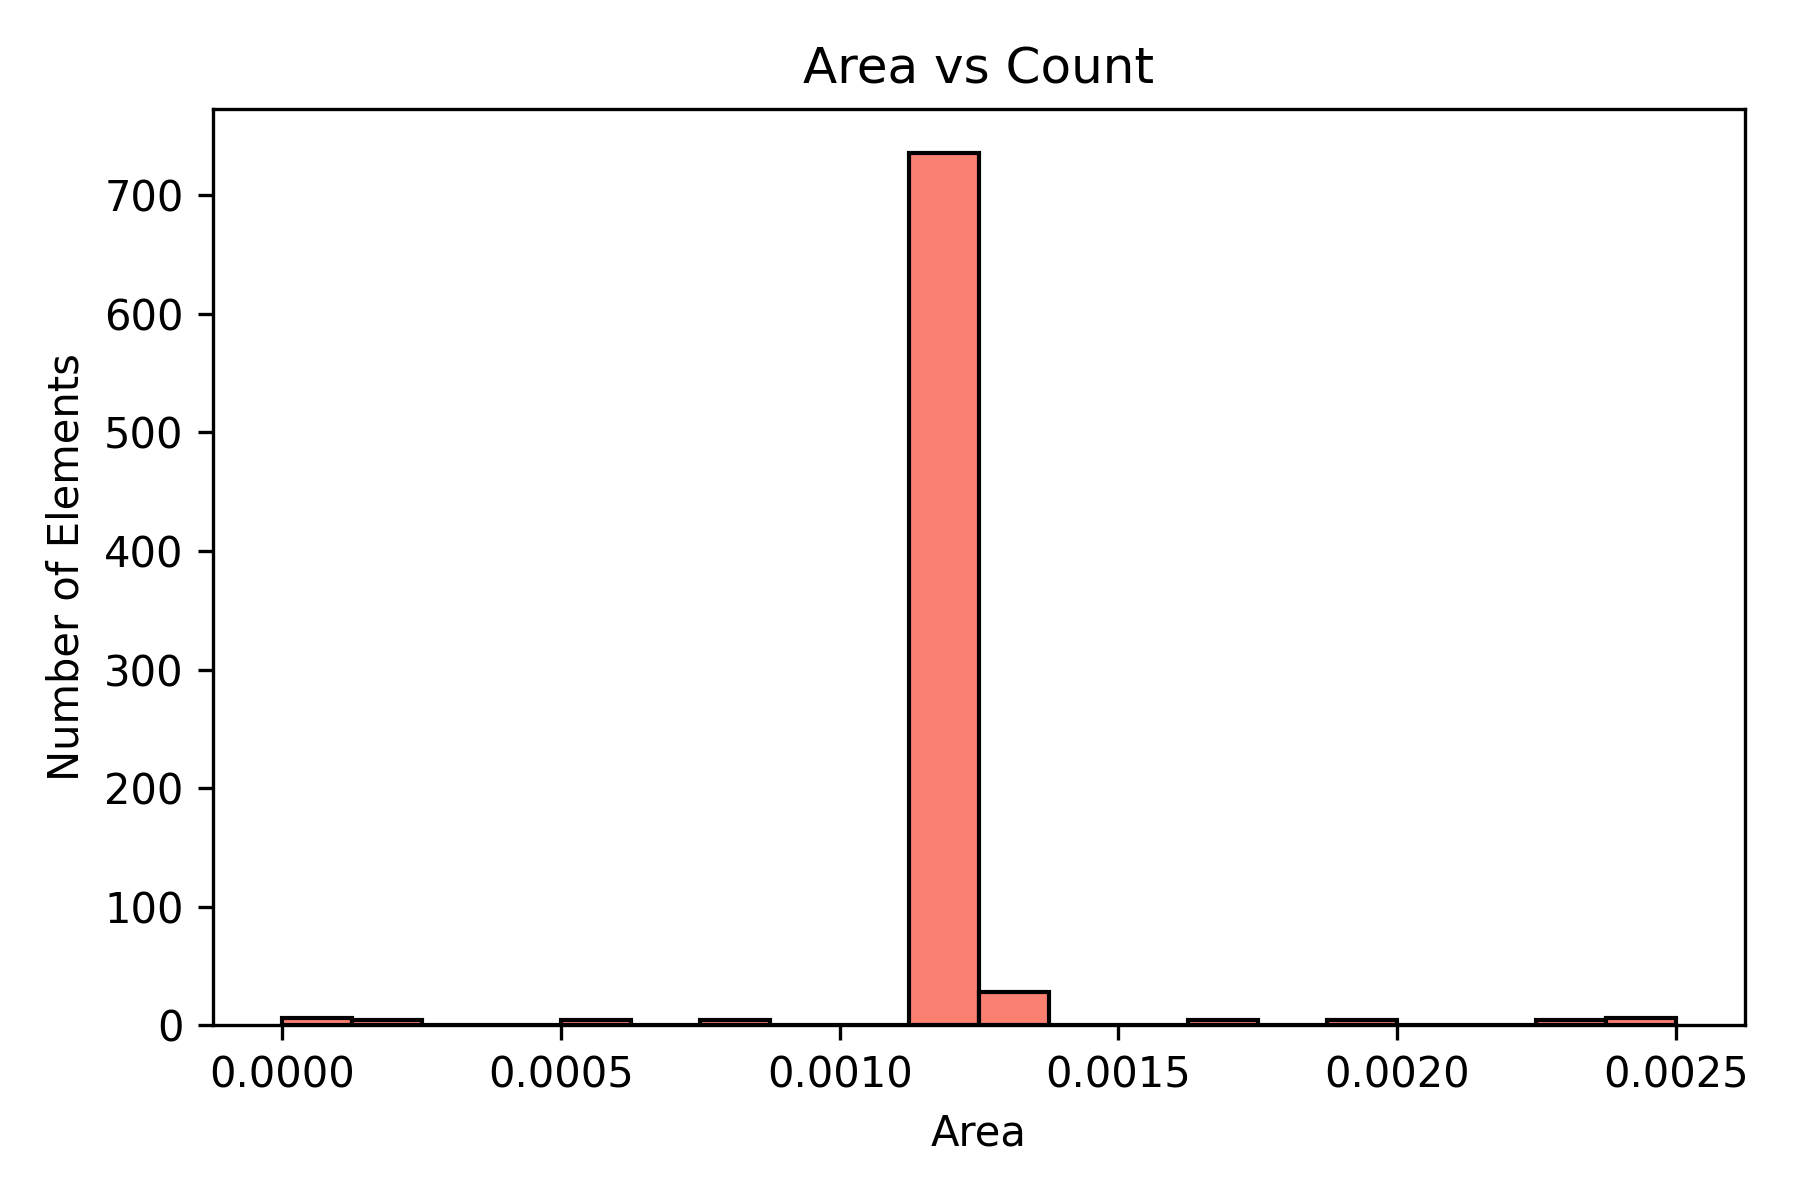
\includegraphics[width=0.55\textwidth]{figures/Figure1.png}
    \caption{Distribution des aires des éléments.}
    \label{fig:area}
\end{figure}
La répartition des aires (Figure \ref{fig:area}) est centrée autour de la valeur nominale, prouvant que la contrainte de volume constant est respectée globalement.

\begin{figure}[H]
    \centering
    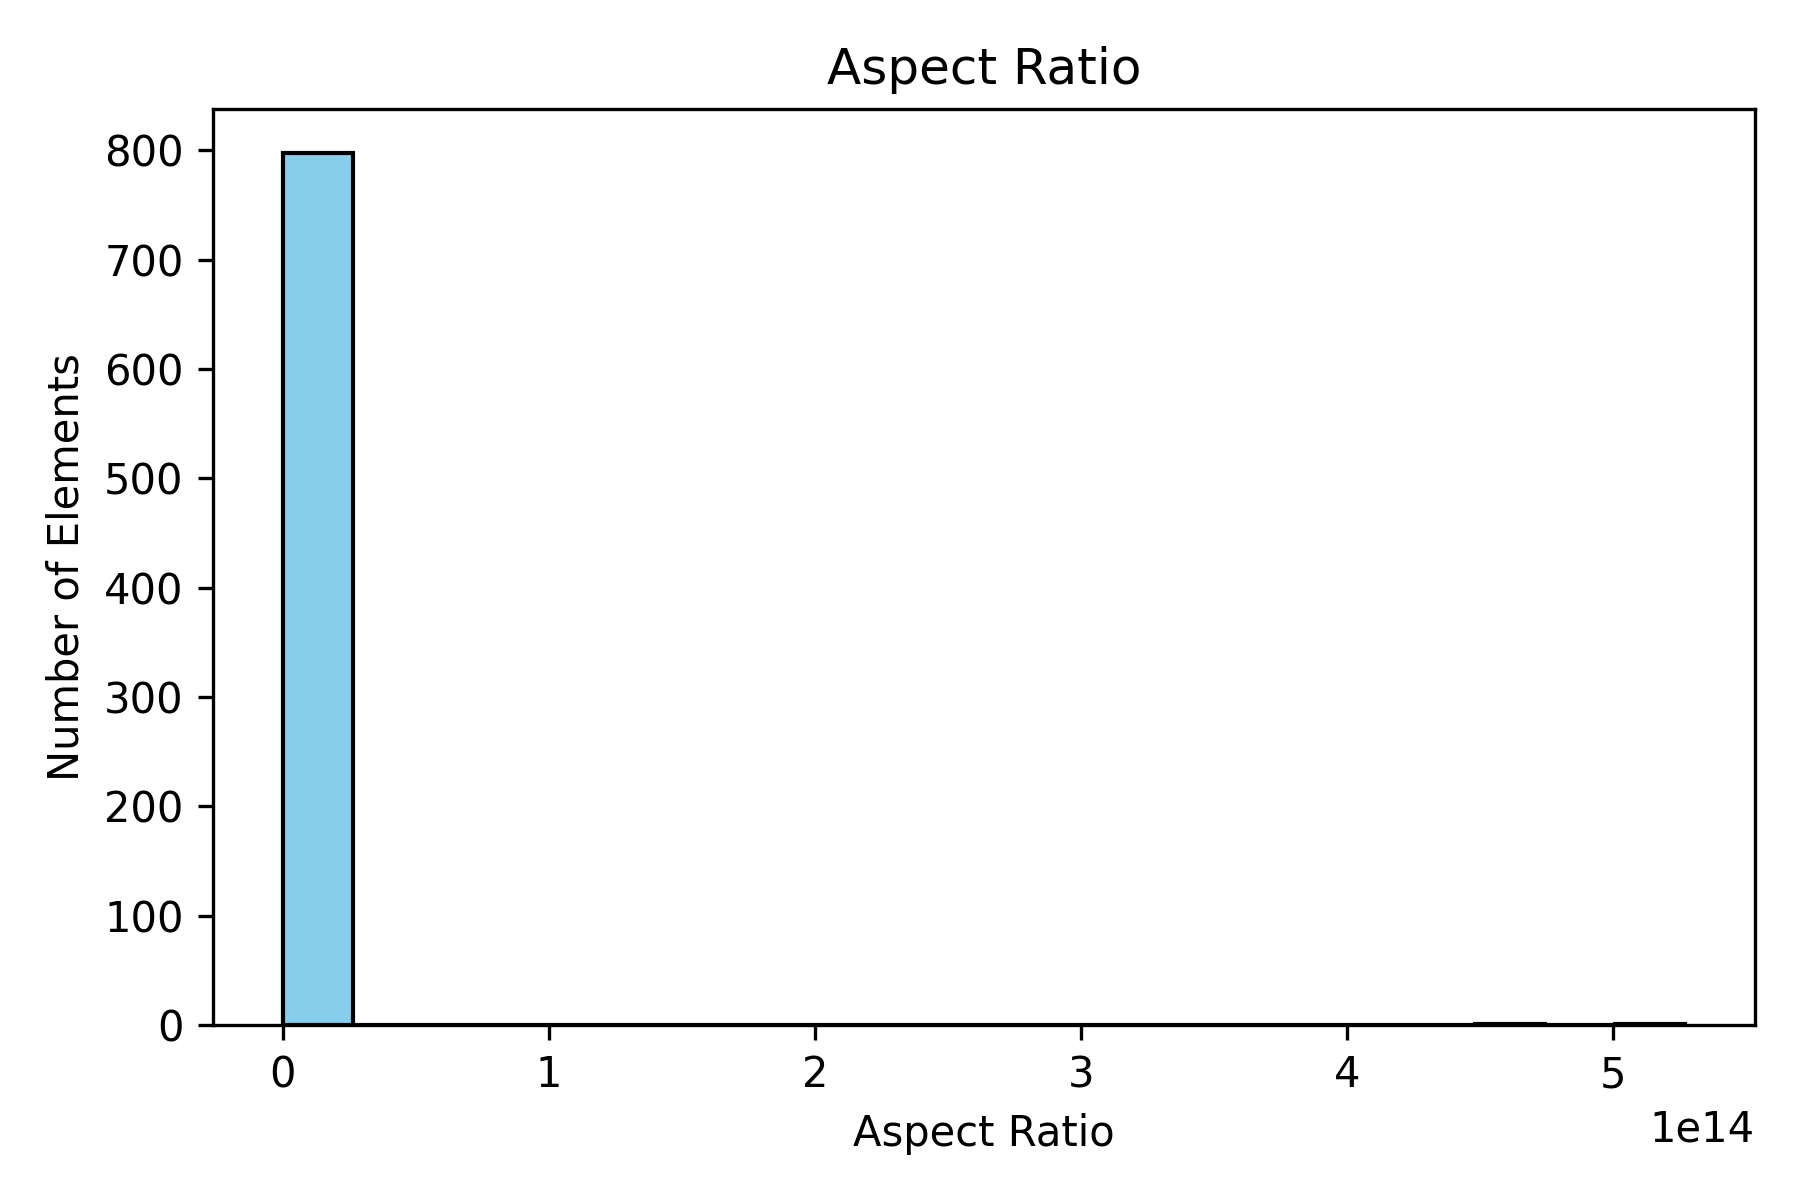
\includegraphics[width=0.55\textwidth]{figures/Figure2.png}
    \caption{Rapport d'aspect des éléments.}
    \label{fig:aspect_ratio}
\end{figure}
Concernant le rapport d'aspect (Figure \ref{fig:aspect_ratio}), la présence de valeurs élevées (\(10^{14}\)) indique une dégénérescence sévère des triangles situés sur la frontière sinusoïdale.

\begin{figure}[H]
    \centering
    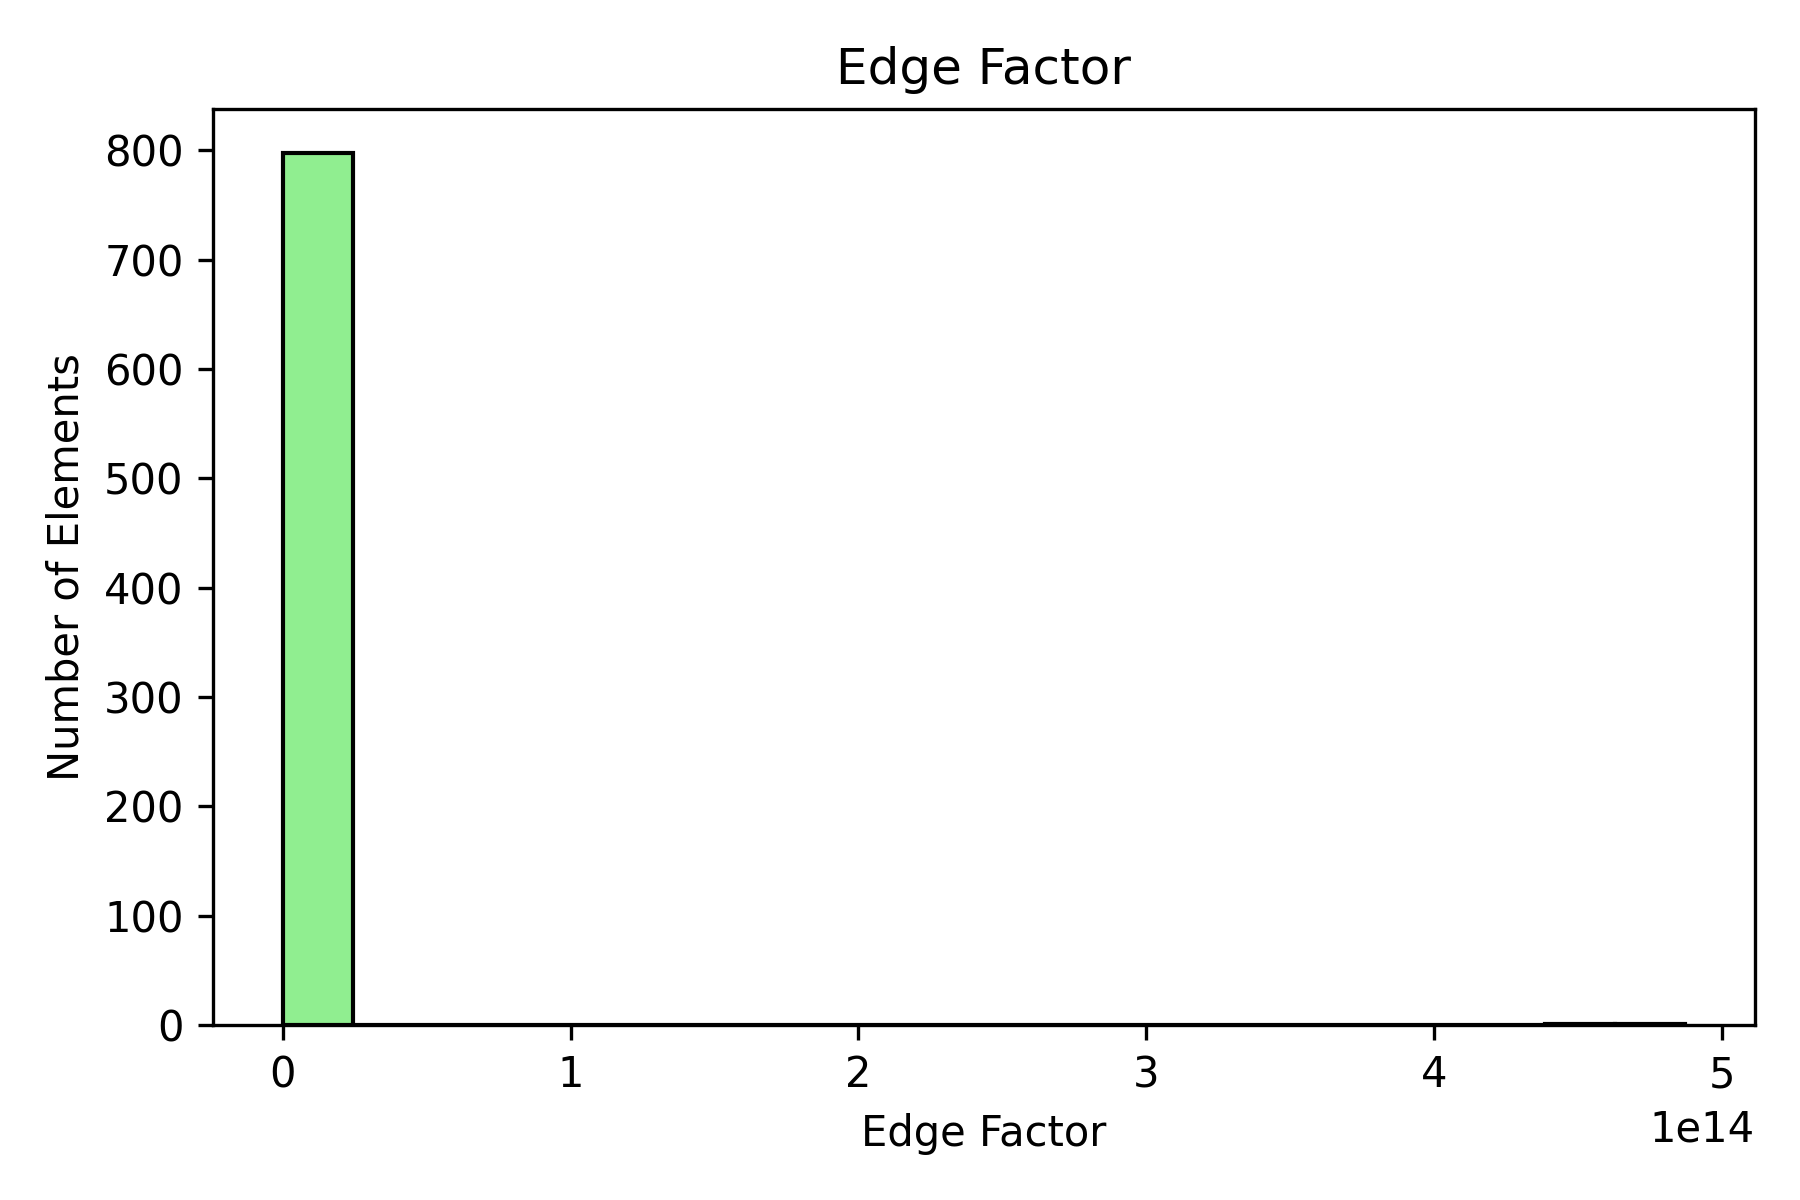
\includegraphics[width=0.55\textwidth]{figures/Figure3.png}
    \caption{Facteur de longueur d'arête.}
    \label{fig:edge_factor}
\end{figure}
La Figure \ref{fig:edge_factor} illustre le rapport d'élongation des arêtes, confirmant les distorsions géométriques locales.

\begin{figure}[H]
    \centering
    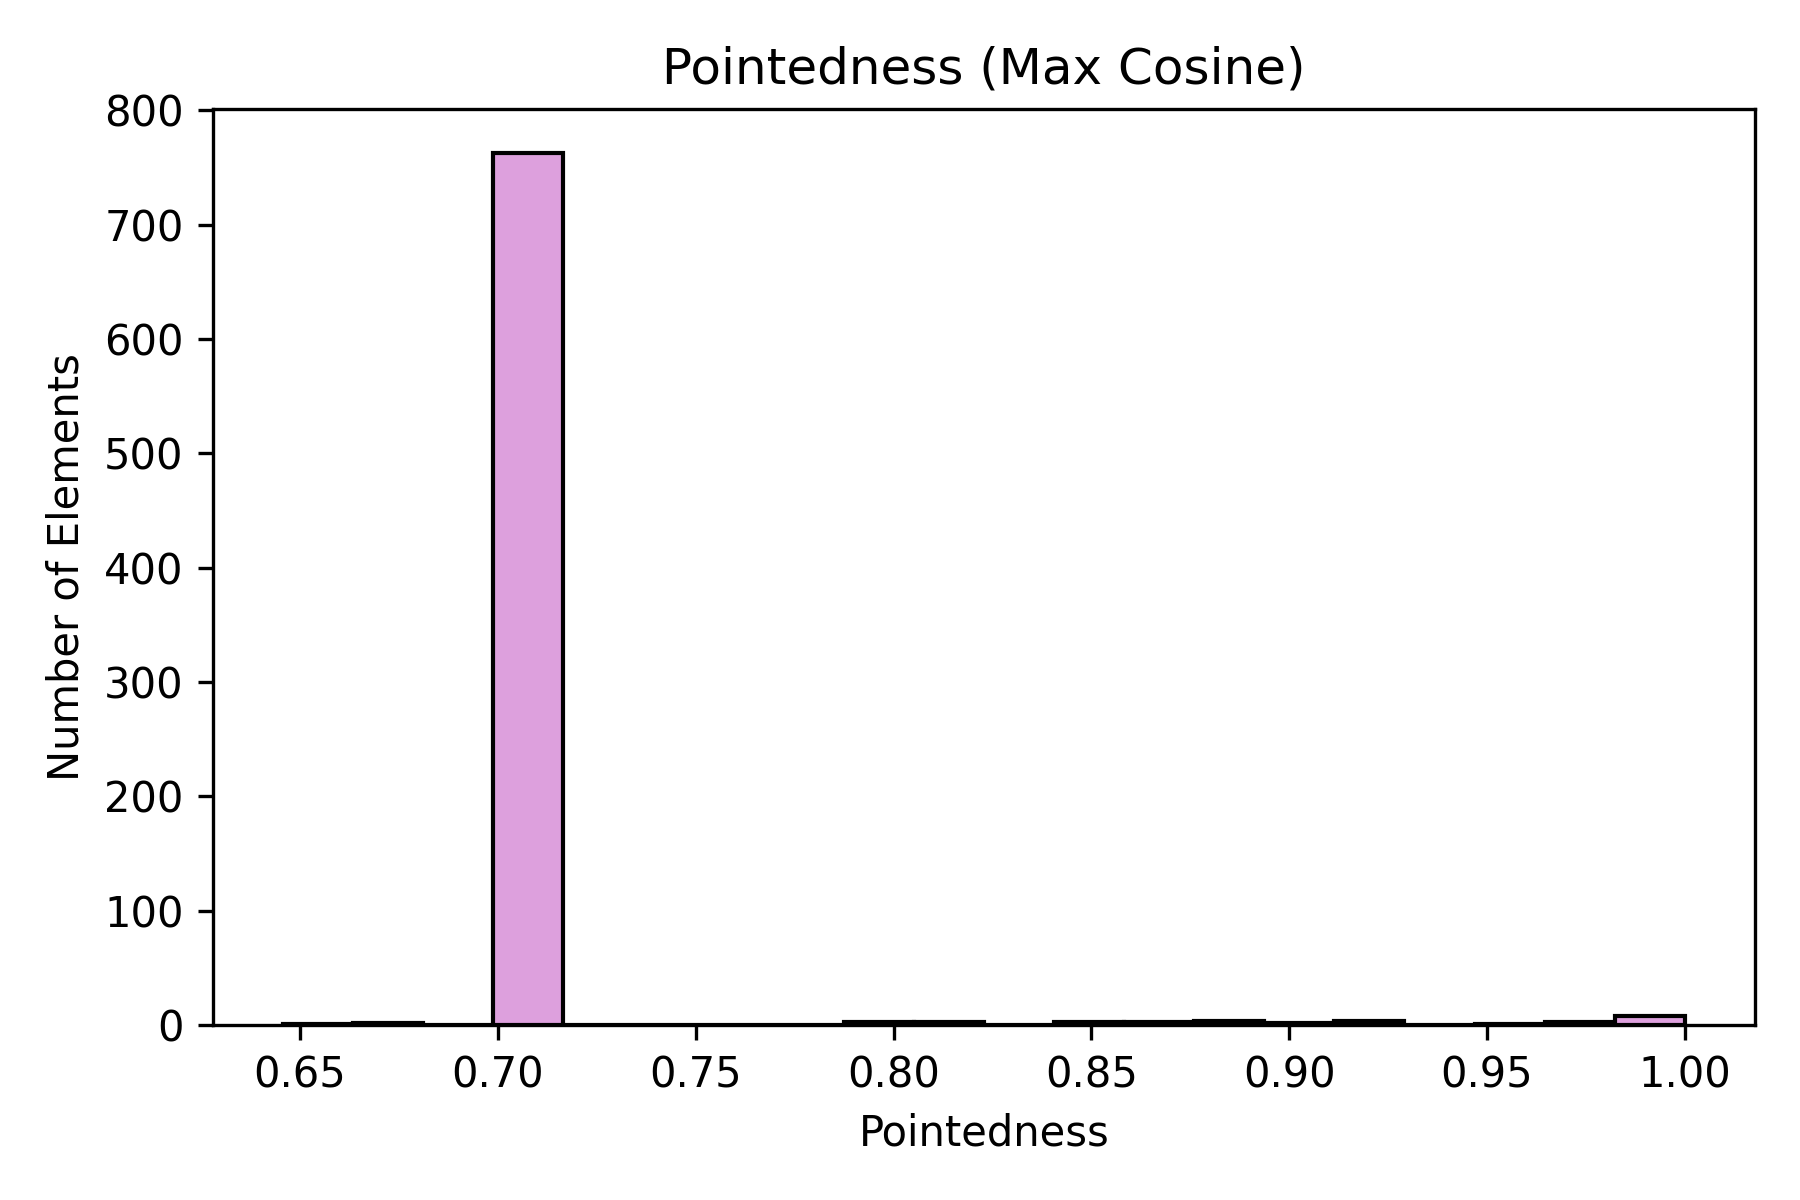
\includegraphics[width=0.55\textwidth]{figures/Figure4.png}
    \caption{Pointu maximal (cosinus).}
    \label{fig:pointedness}
\end{figure}
Enfin, pour le pointu maximal (Figure \ref{fig:pointedness}), certains triangles frôlent un angle plat (\(\cos \approx 1.0\)), impactant directement le conditionnement des matrices FEM.

\section{Précision de la méthode des éléments finis}

\subsection{Modélisation mathématique et formulation faible}
Le problème acoustique est régi par l'équation de Helmholtz :
\begin{equation}
(-\Delta - k^{2})u = f \quad \text{dans } \Omega
\end{equation}
En multipliant par une fonction test \(v \in H^1_0(\Omega)\) et en appliquant la première identité de Green, le terme de bord s'annule et l'on obtient la formulation faible :
\begin{equation}
\text{Trouver } u \in H^1(\Omega) \text{ tel que } \forall v \in H^1_0(\Omega), \quad \int_{\Omega} \nabla u \cdot \nabla v \, dx - k^2 \int_{\Omega} uv \, dx = \int_{\Omega} fv \, dx
\end{equation}

\subsection{Implémentation FEM et matrices creuses}
La discrétisation par éléments \(P_1\) conduit au système algébrique \((K - k^2 M)u_h = F\). L'assemblage utilise des \textbf{matrices creuses} (\texttt{scipy.sparse}). Les conditions de Dirichlet sont imposées fortement avec report de l'influence sur le second membre. 

\subsection{Étude théorique et normes d'erreur}
L'erreur numérique \(err = ||u^{*} - u_{h}||\) est évaluée rigoureusement à travers trois métriques : la norme \(L_2\) (pondérée par \(h\)), la norme du supremum \(L_\infty\) (erreur maximale) et la semi-norme \(H^1\). La borne théorique s'écrit :
\begin{equation}
||u^{*} - u_{h}|| \le C_1 h^\alpha + C_2 k^\beta h^\alpha
\end{equation}
où le terme en \(k^\beta h^\alpha\) traduit la pollution numérique due au déphasage cumulé de l'onde.

\section{Analyse des résultats empiriques}

\subsection{Cas du maillage régulier}
L'exécution sur le maillage de référence (\(16 \times 4\) avec \(k=\pi\)) a validé les erreurs initiales suivantes : norme \(L_2 = 3.88 \times 10^{-3}\), norme \(L_\infty = 3.57 \times 10^{-3}\) et semi-norme \(H^1 = 1.51 \times 10^{-2}\).

\begin{figure}[H]
    \centering
    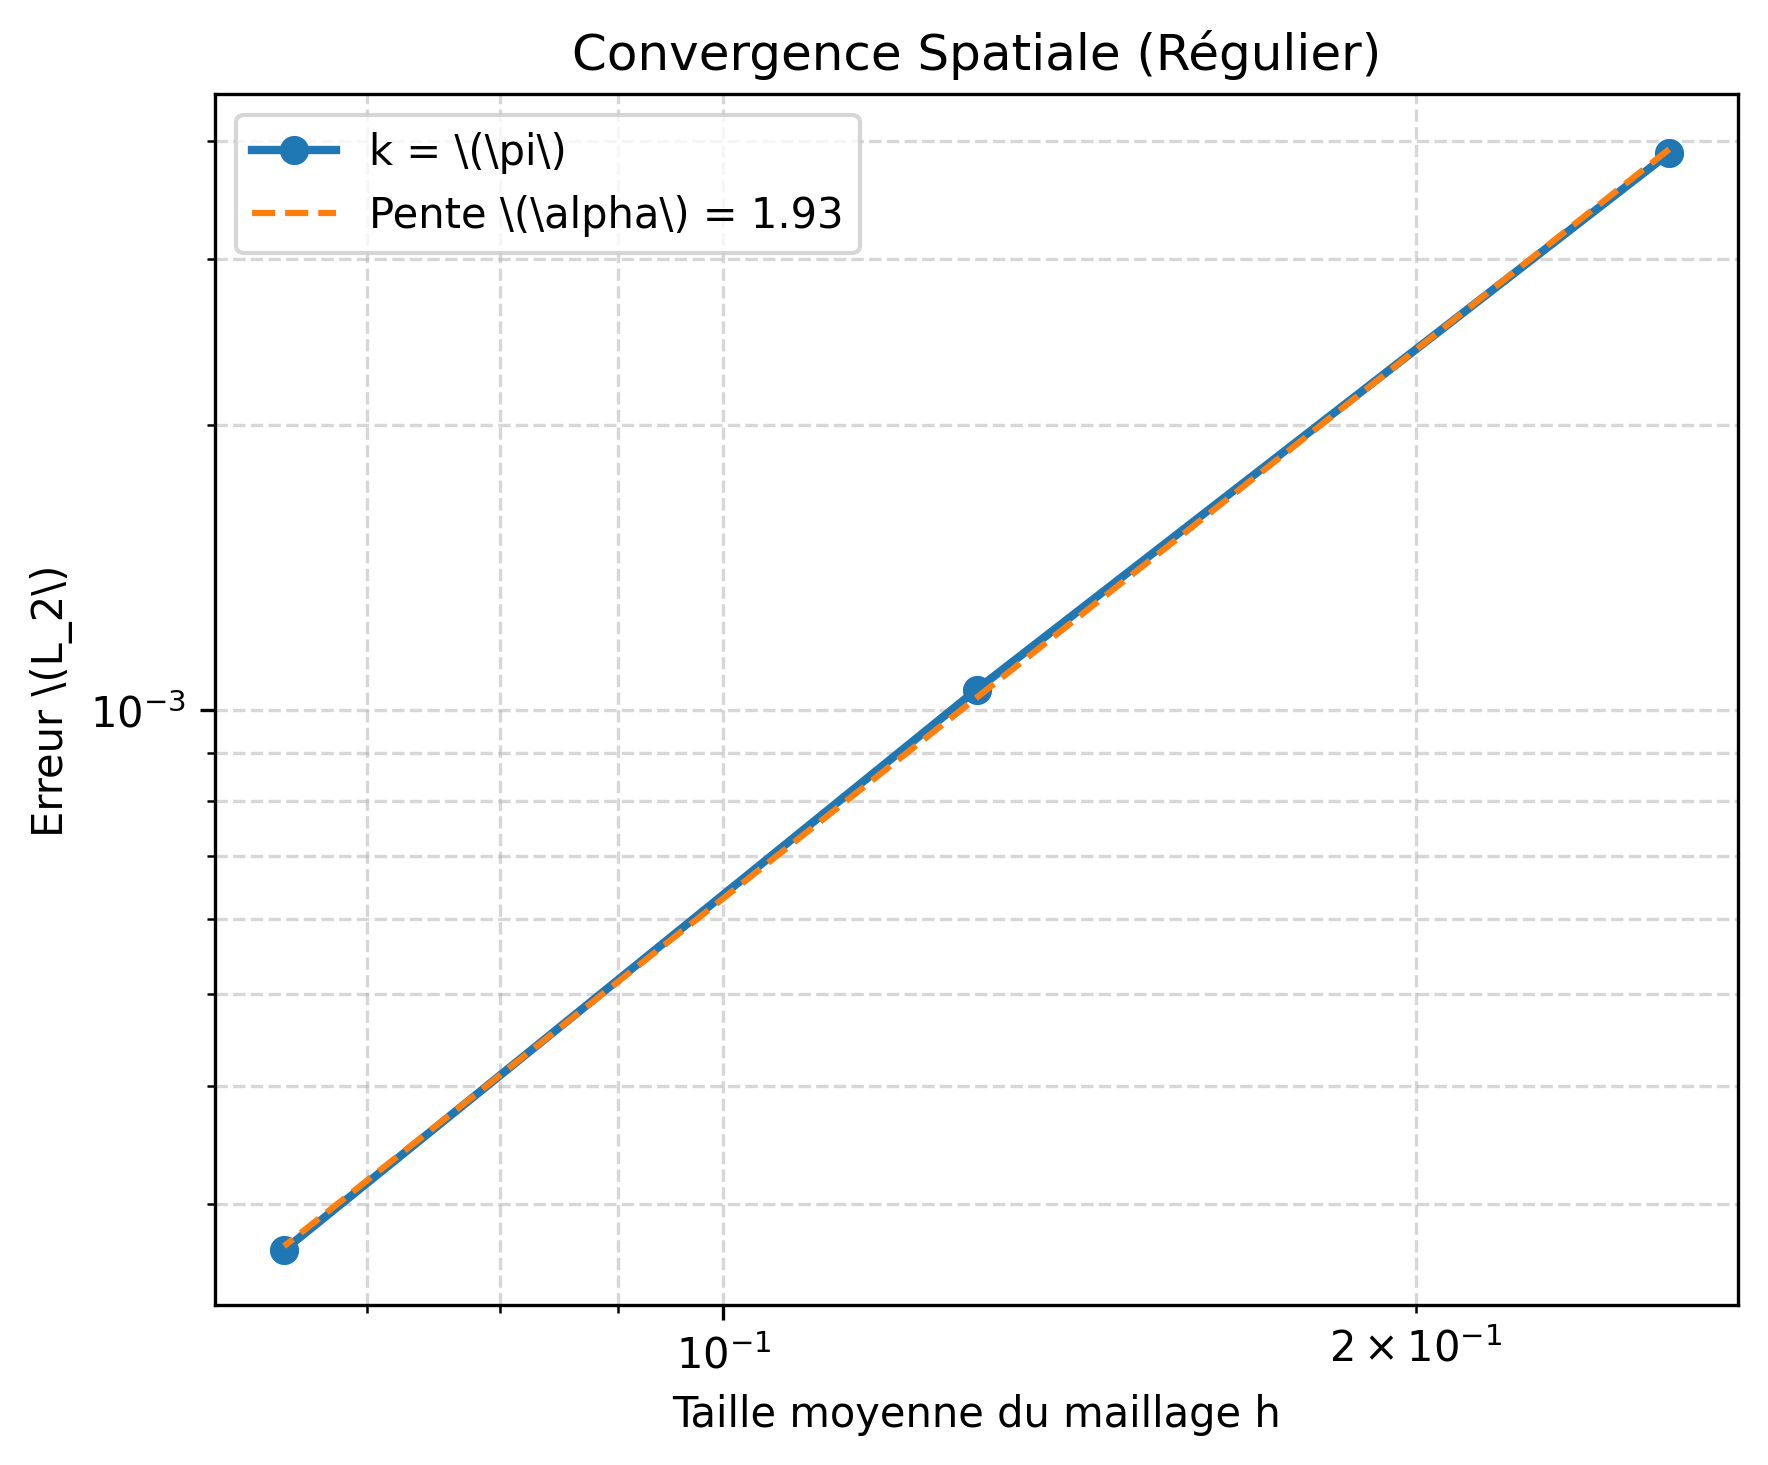
\includegraphics[width=0.55\textwidth]{figures/Figure5.png}
    \caption{Convergence spatiale (maillage régulier).}
    \label{fig:c5}
\end{figure}
La régression log-log (Figure \ref{fig:c5}) donne une pente \(\alpha = 1.93\), en adéquation étroite avec la théorie des éléments \(P_1\) (\(\alpha = 2\)).

\begin{figure}[H]
    \centering
    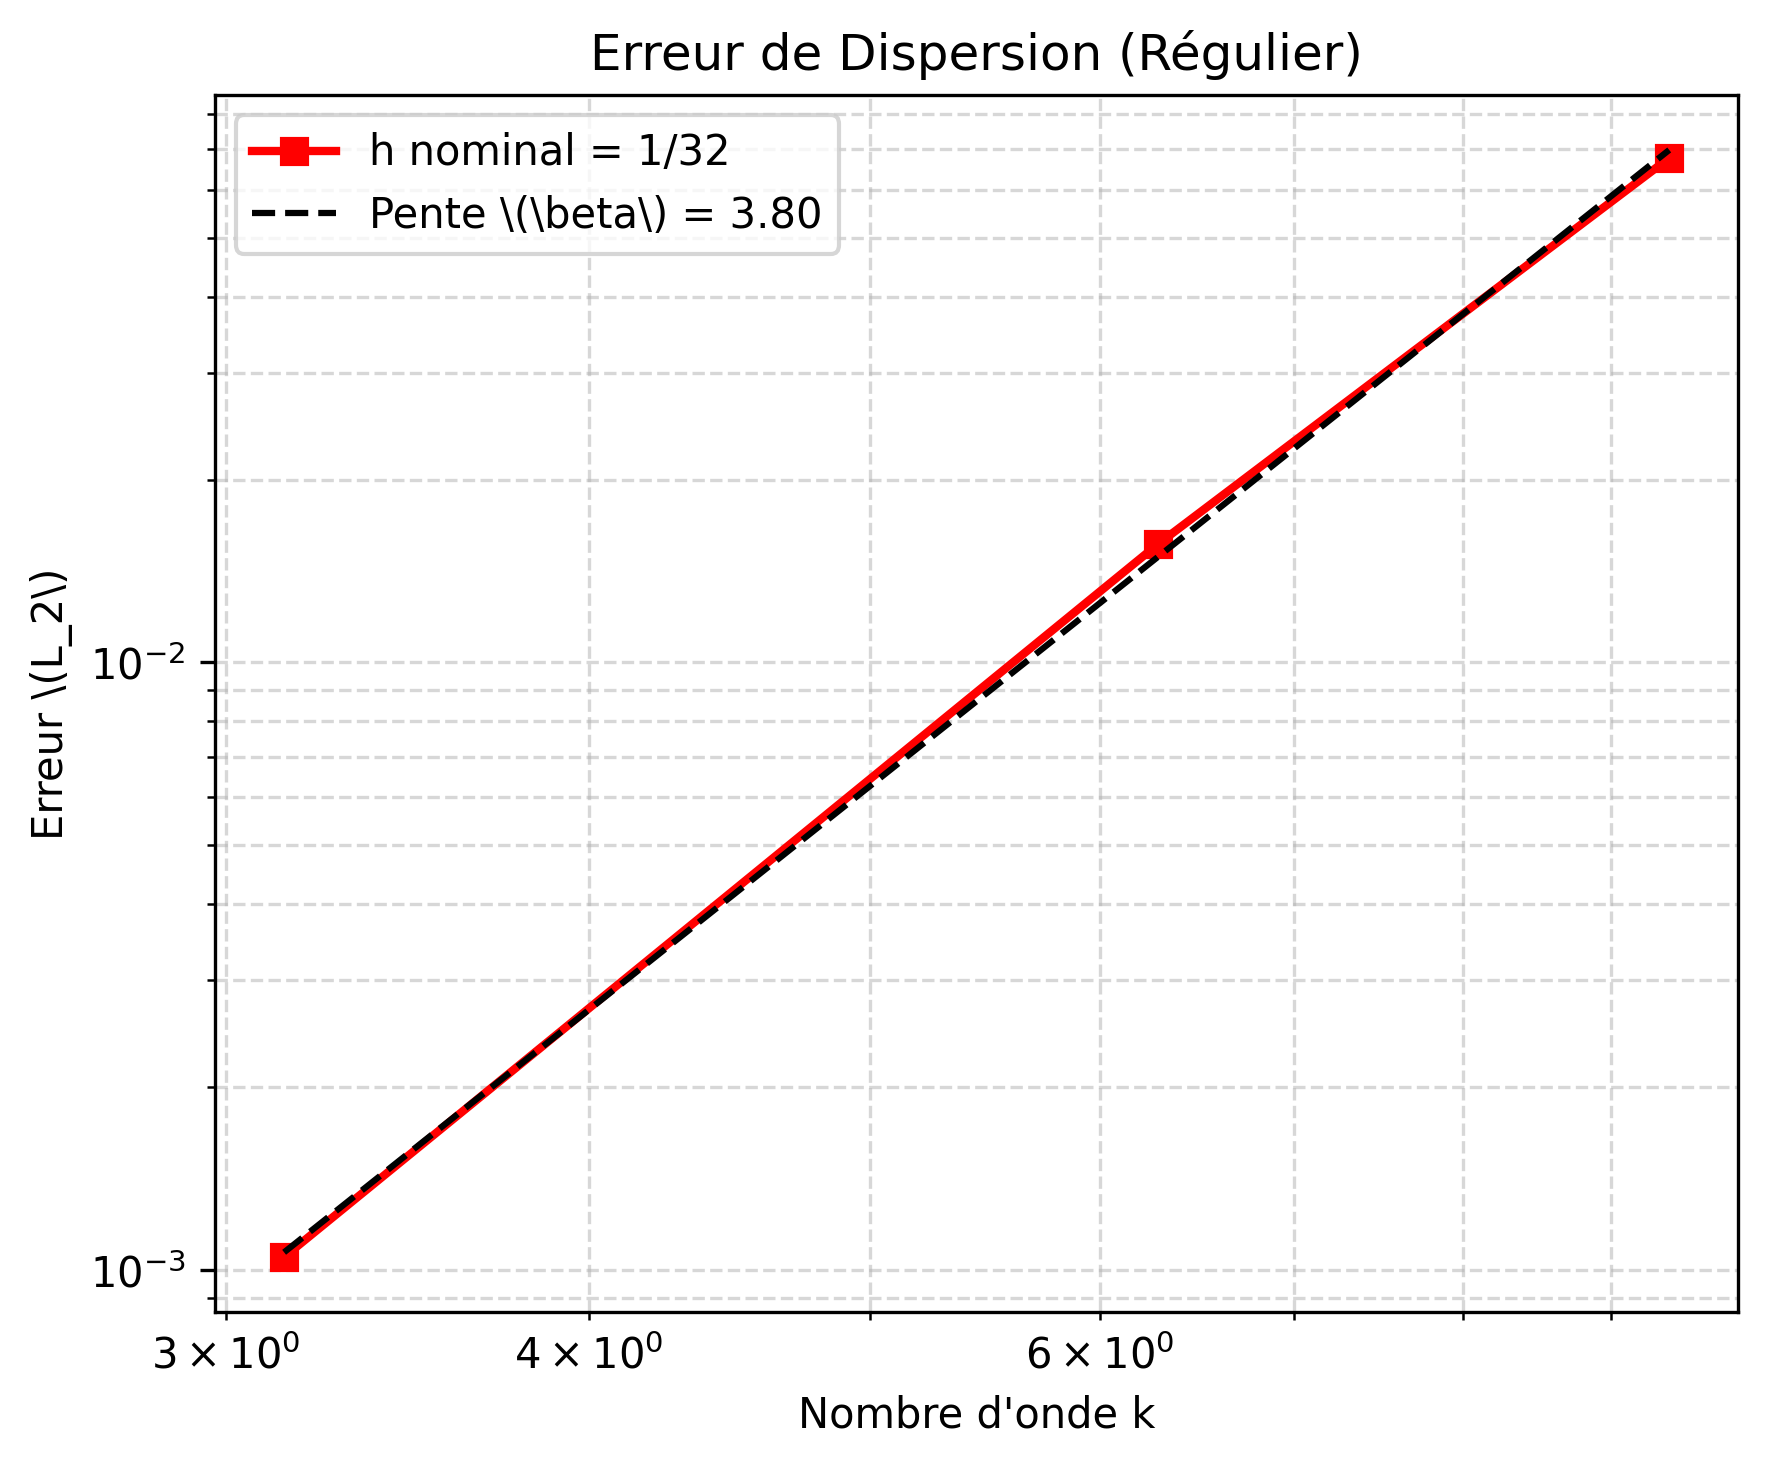
\includegraphics[width=0.55\textwidth]{figures/Figure6.png}
    \caption{Erreur de dispersion (maillage régulier).}
    \label{fig:c6}
\end{figure}
La Figure \ref{fig:c6} met en évidence la croissance de l'erreur avec \(k\), menant à une évaluation empirique de \(\beta = 3.80\).

\begin{figure}[H]
    \centering
    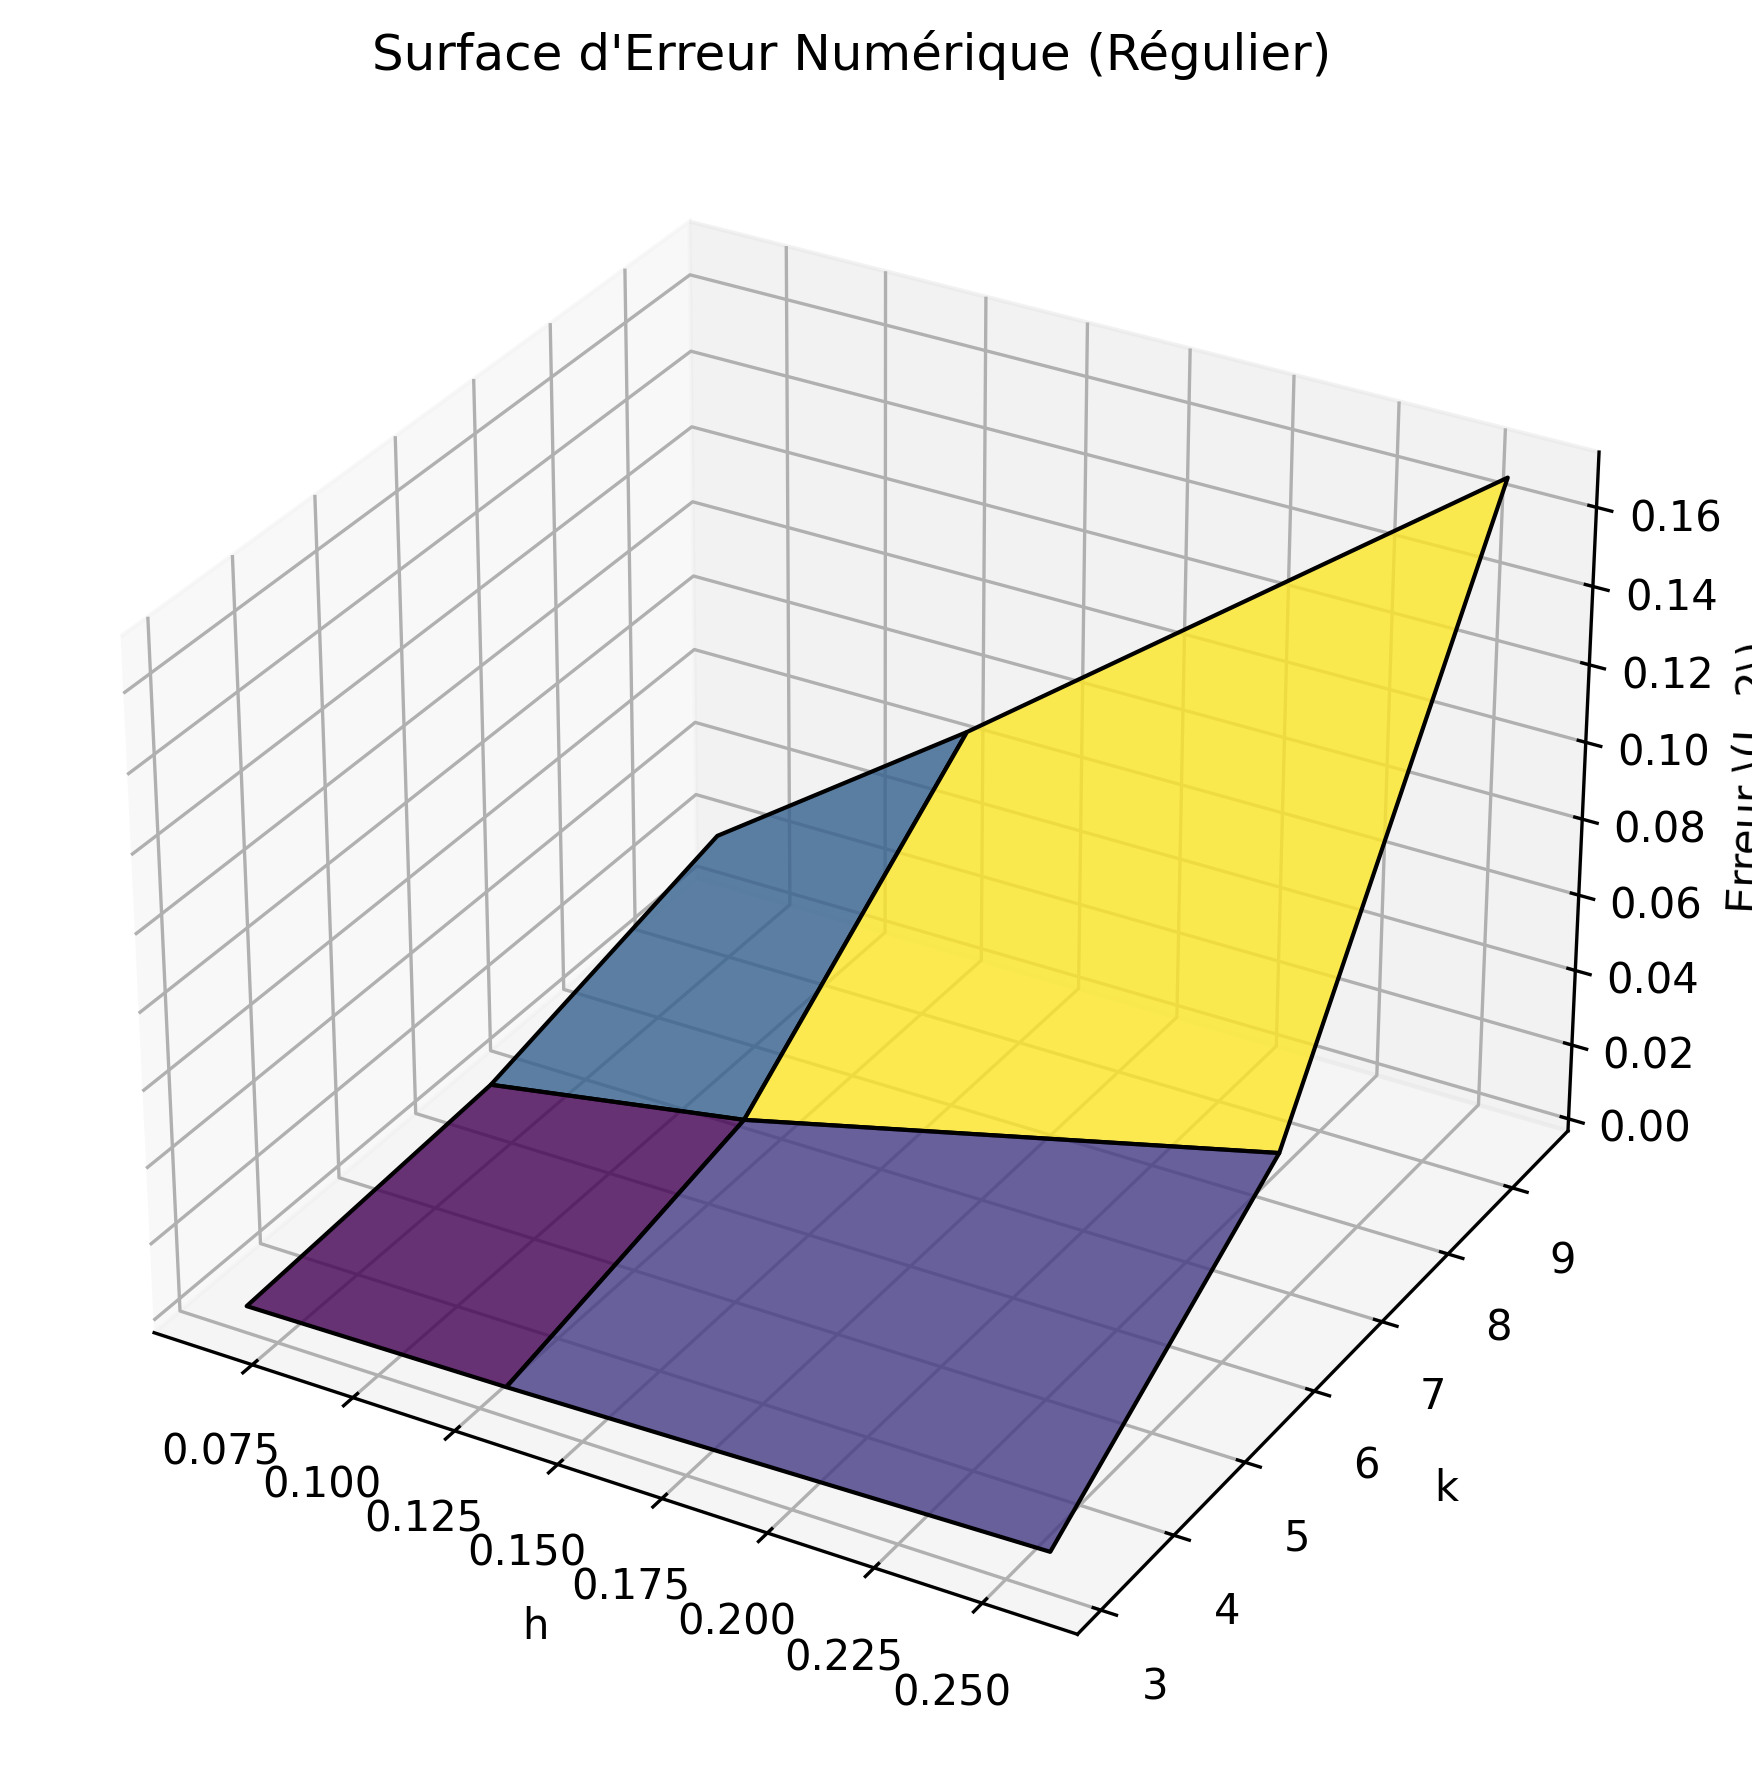
\includegraphics[width=0.55\textwidth]{figures/Figure7.png}
    \caption{Surface tridimensionnelle d'erreur (maillage régulier).}
    \label{fig:c7}
\end{figure}
La vue tridimensionnelle (Figure \ref{fig:c7}) illustre la sensibilité conjointe de la solution face au raffinement \(h\) et à la fréquence \(k\).

\begin{figure}[H]
    \centering
    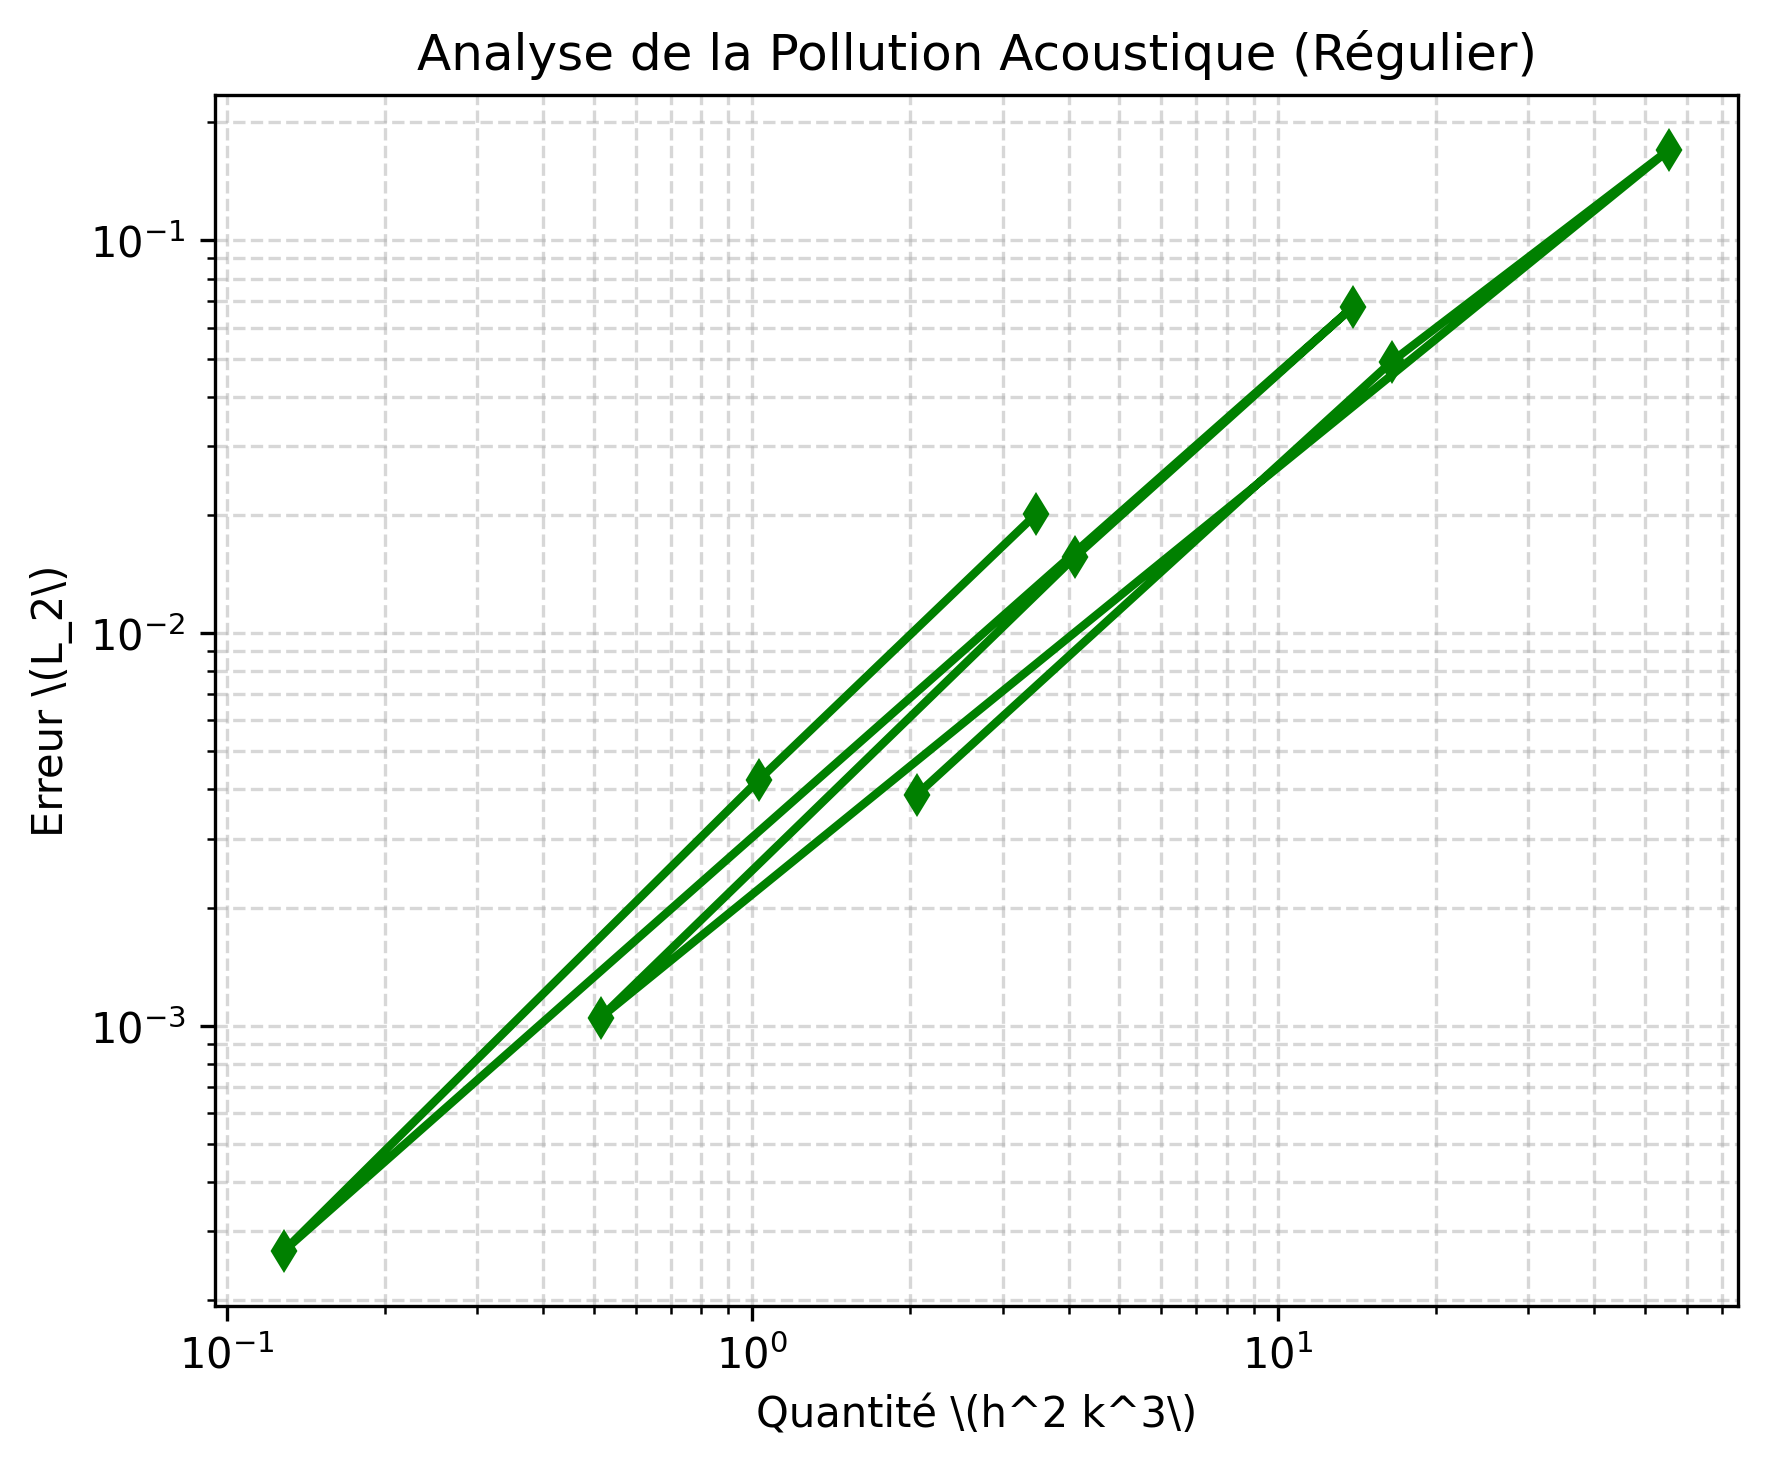
\includegraphics[width=0.55\textwidth]{figures/Figure8.png}
    \caption{Analyse de la pollution \(h^2 k^3\) (maillage régulier).}
    \label{fig:c8}
\end{figure}
La Figure \ref{fig:c8} démontre le régime asymptotique où la dispersion domine l'interpolation géométrique.

\subsection{Cas du maillage déformé (shifté)}
Conformément à la seconde partie du projet, l'étude a été réitérée sur le maillage dont les nœuds internes ont subi un déplacement adaptatif (shift).

\begin{figure}[H]
    \centering
    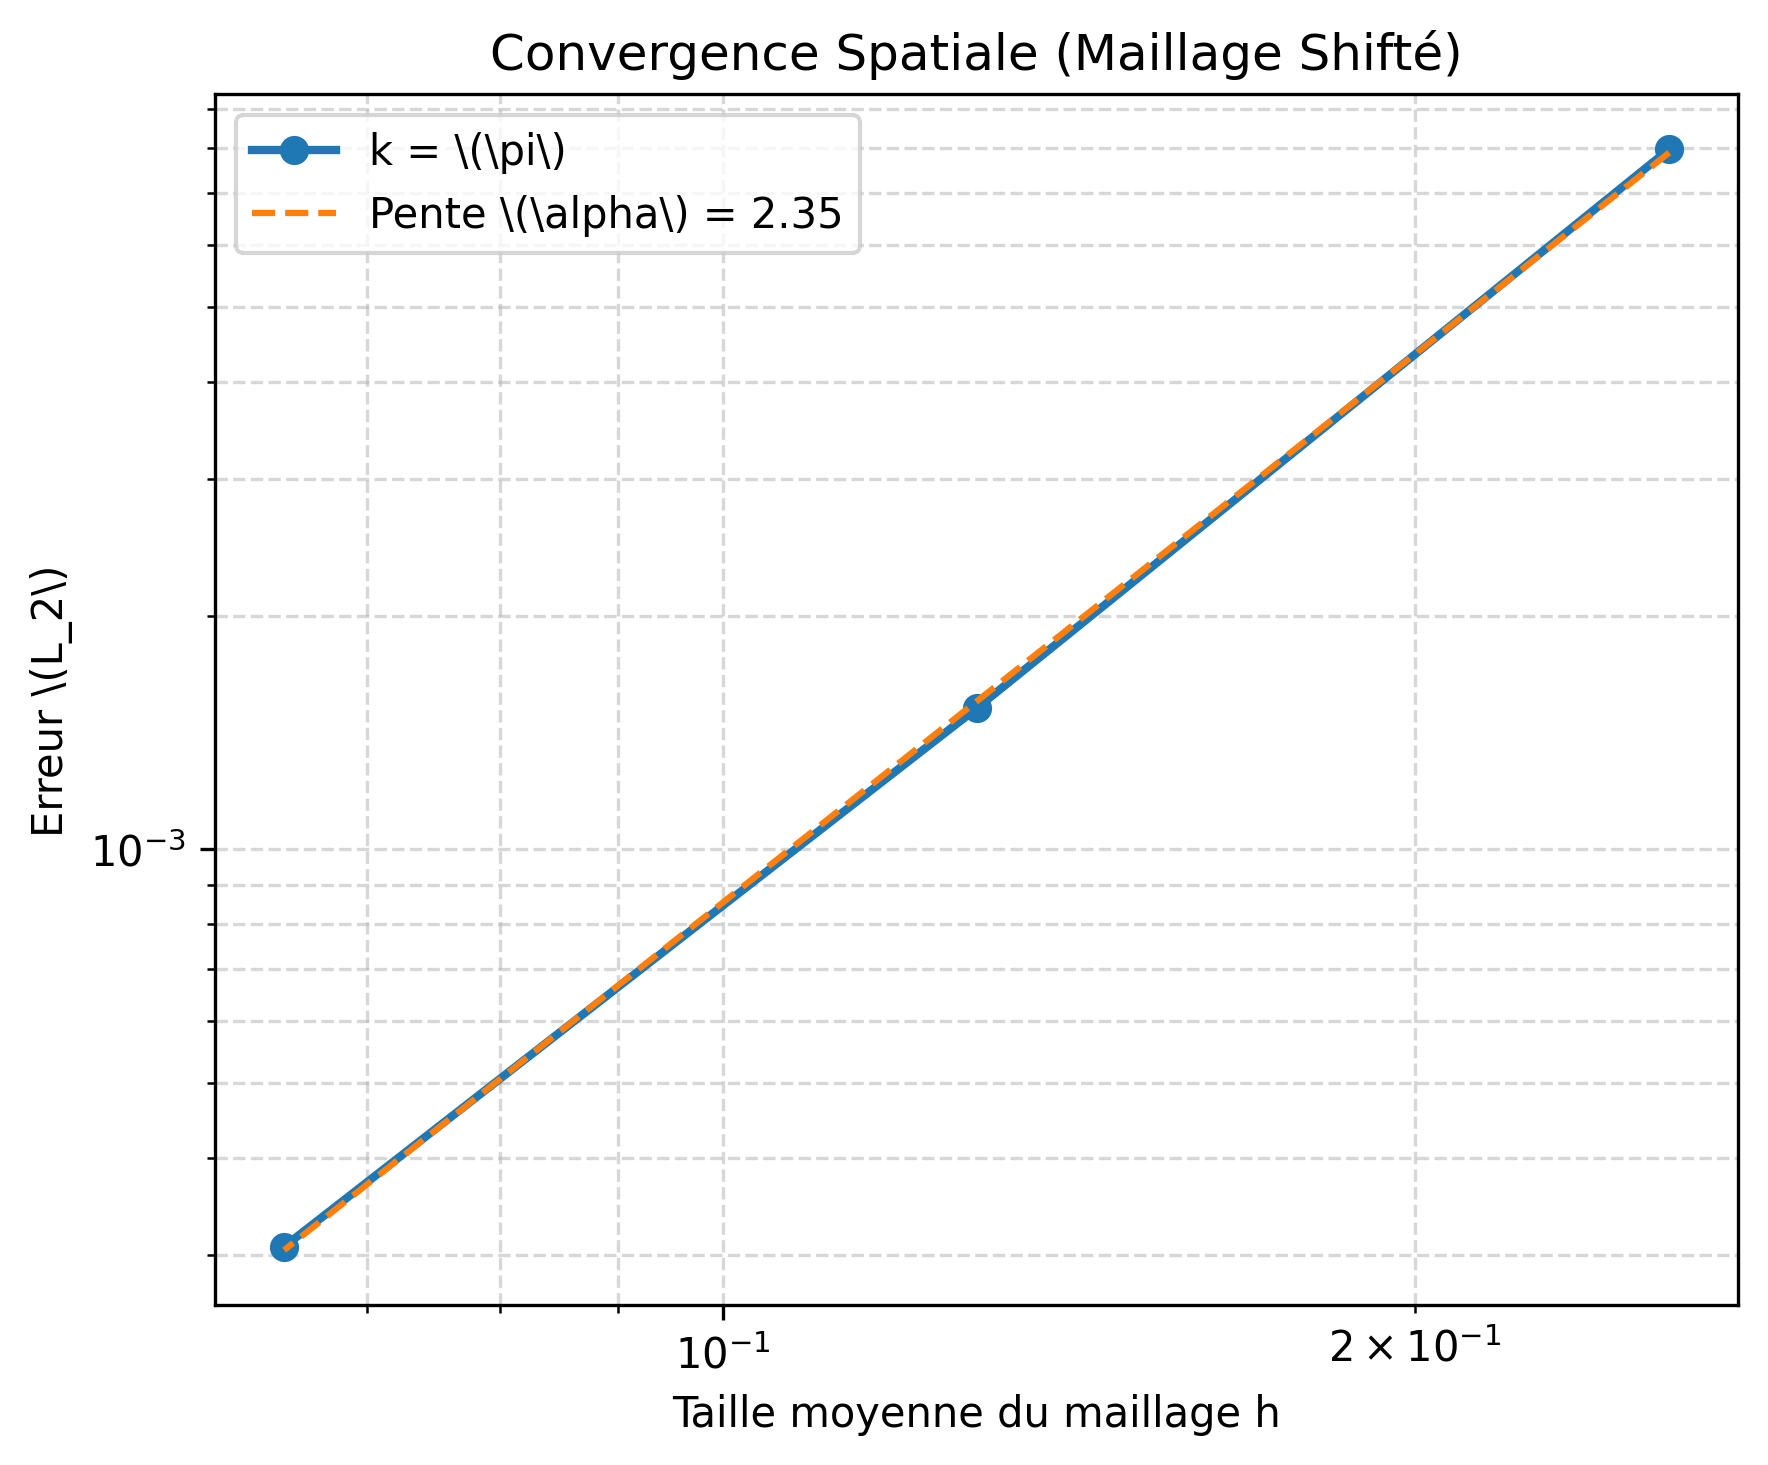
\includegraphics[width=0.55\textwidth]{figures/Figure9.png}
    \caption{Convergence spatiale (maillage shifté).}
    \label{fig:c9}
\end{figure}
Sur ce maillage déformé, le taux de convergence spatiale global atteint \(\alpha = 2.35\) (Figure \ref{fig:c9}), ce qui reflète une sensibilité locale de l'estimation de pente due aux distorsions.

\begin{figure}[H]
    \centering
    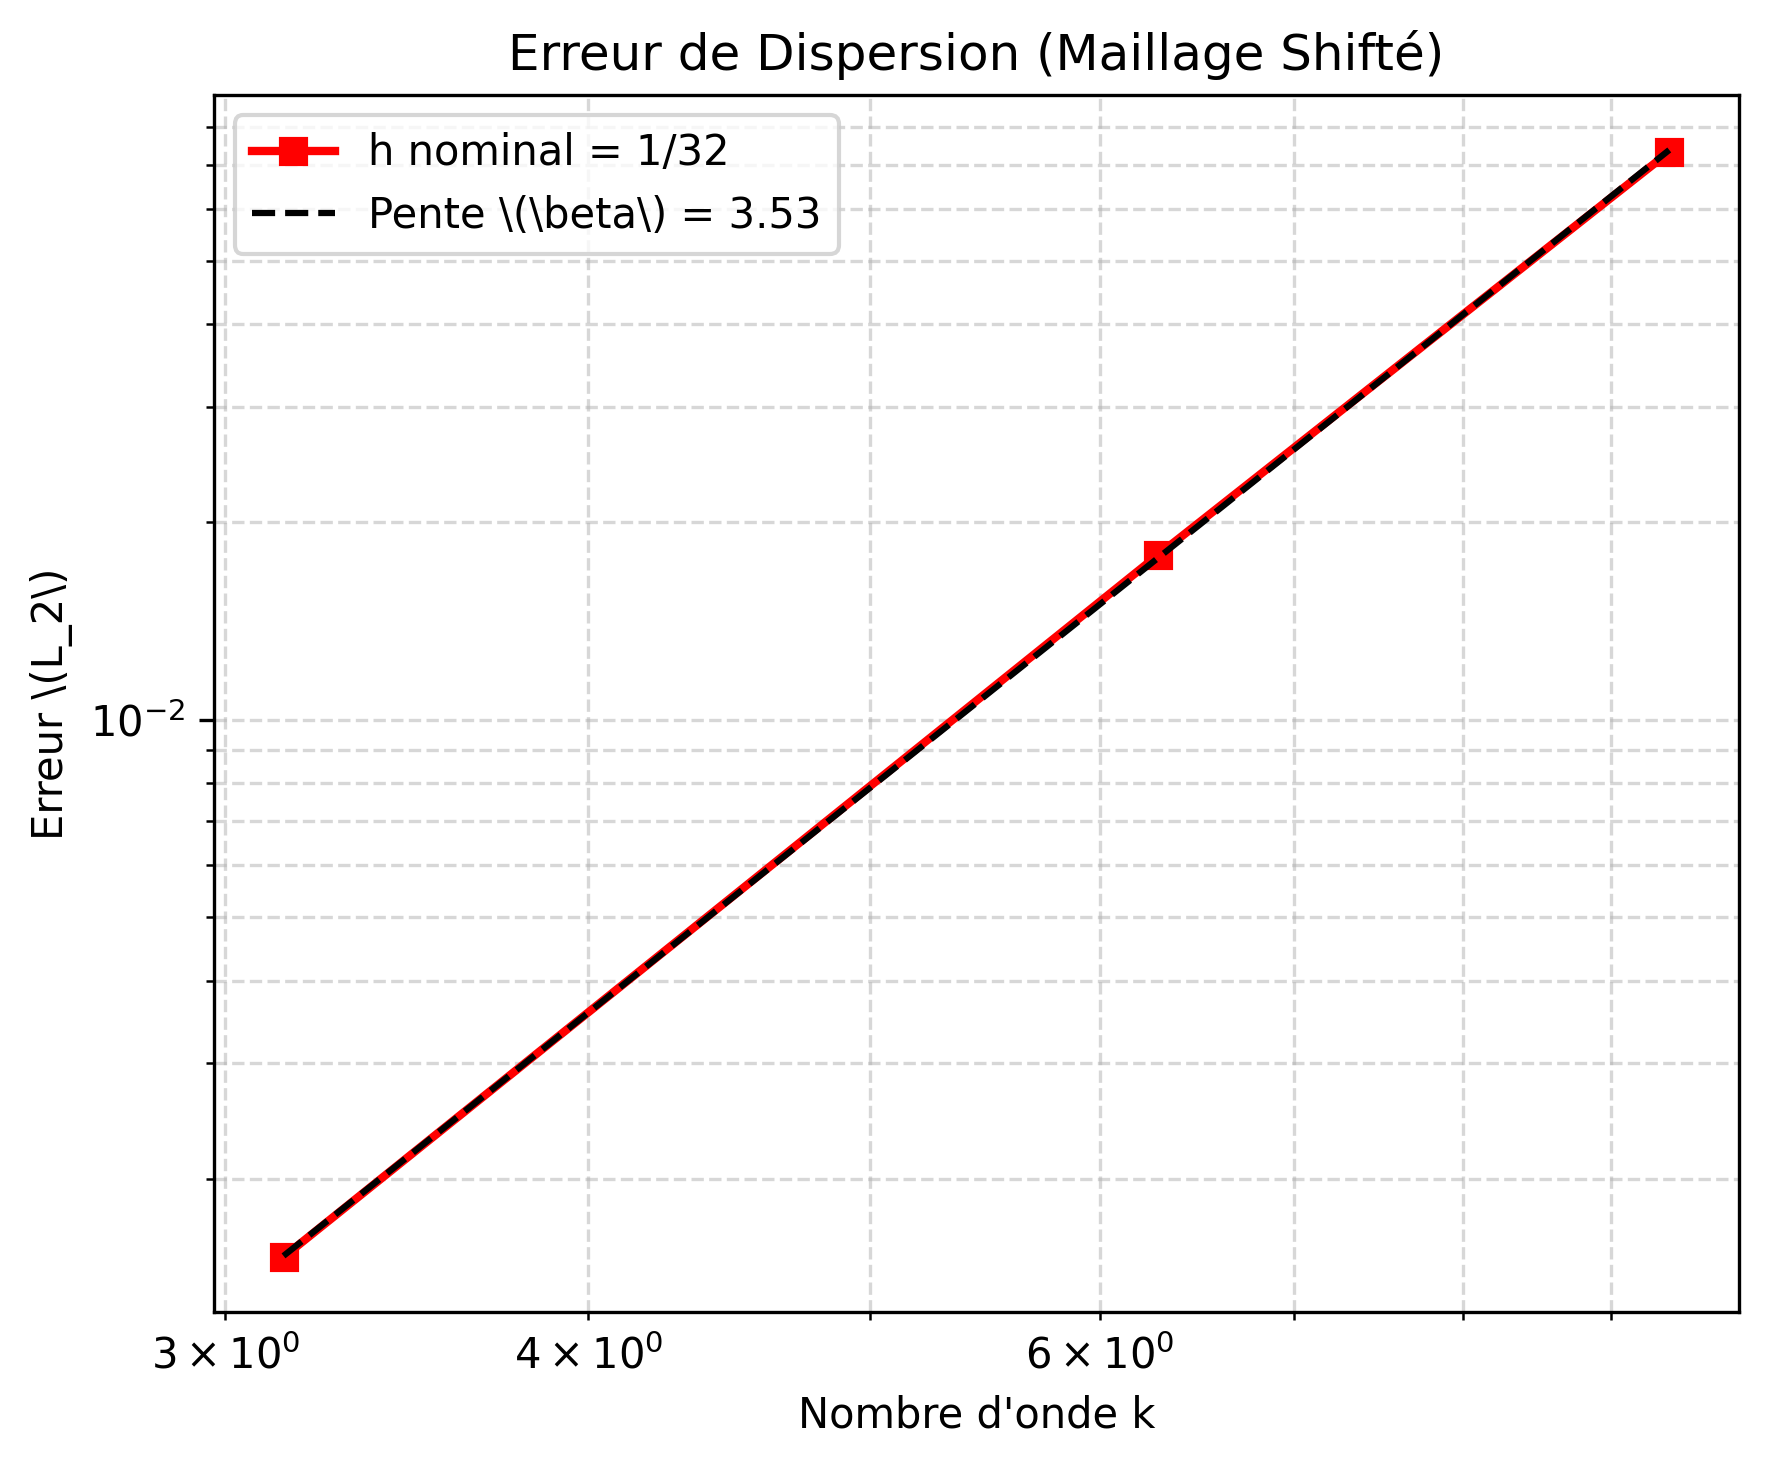
\includegraphics[width=0.55\textwidth]{figures/Figure10.png}
    \caption{Erreur de dispersion (maillage shifté).}
    \label{fig:c10}
\end{figure}
L'erreur de dispersion (Figure \ref{fig:c10}) évalue un paramètre de dispersion \(\beta = 3.53\), confirmant la robustesse de la croissance de l'erreur en fréquence.

\begin{figure}[H]
    \centering
    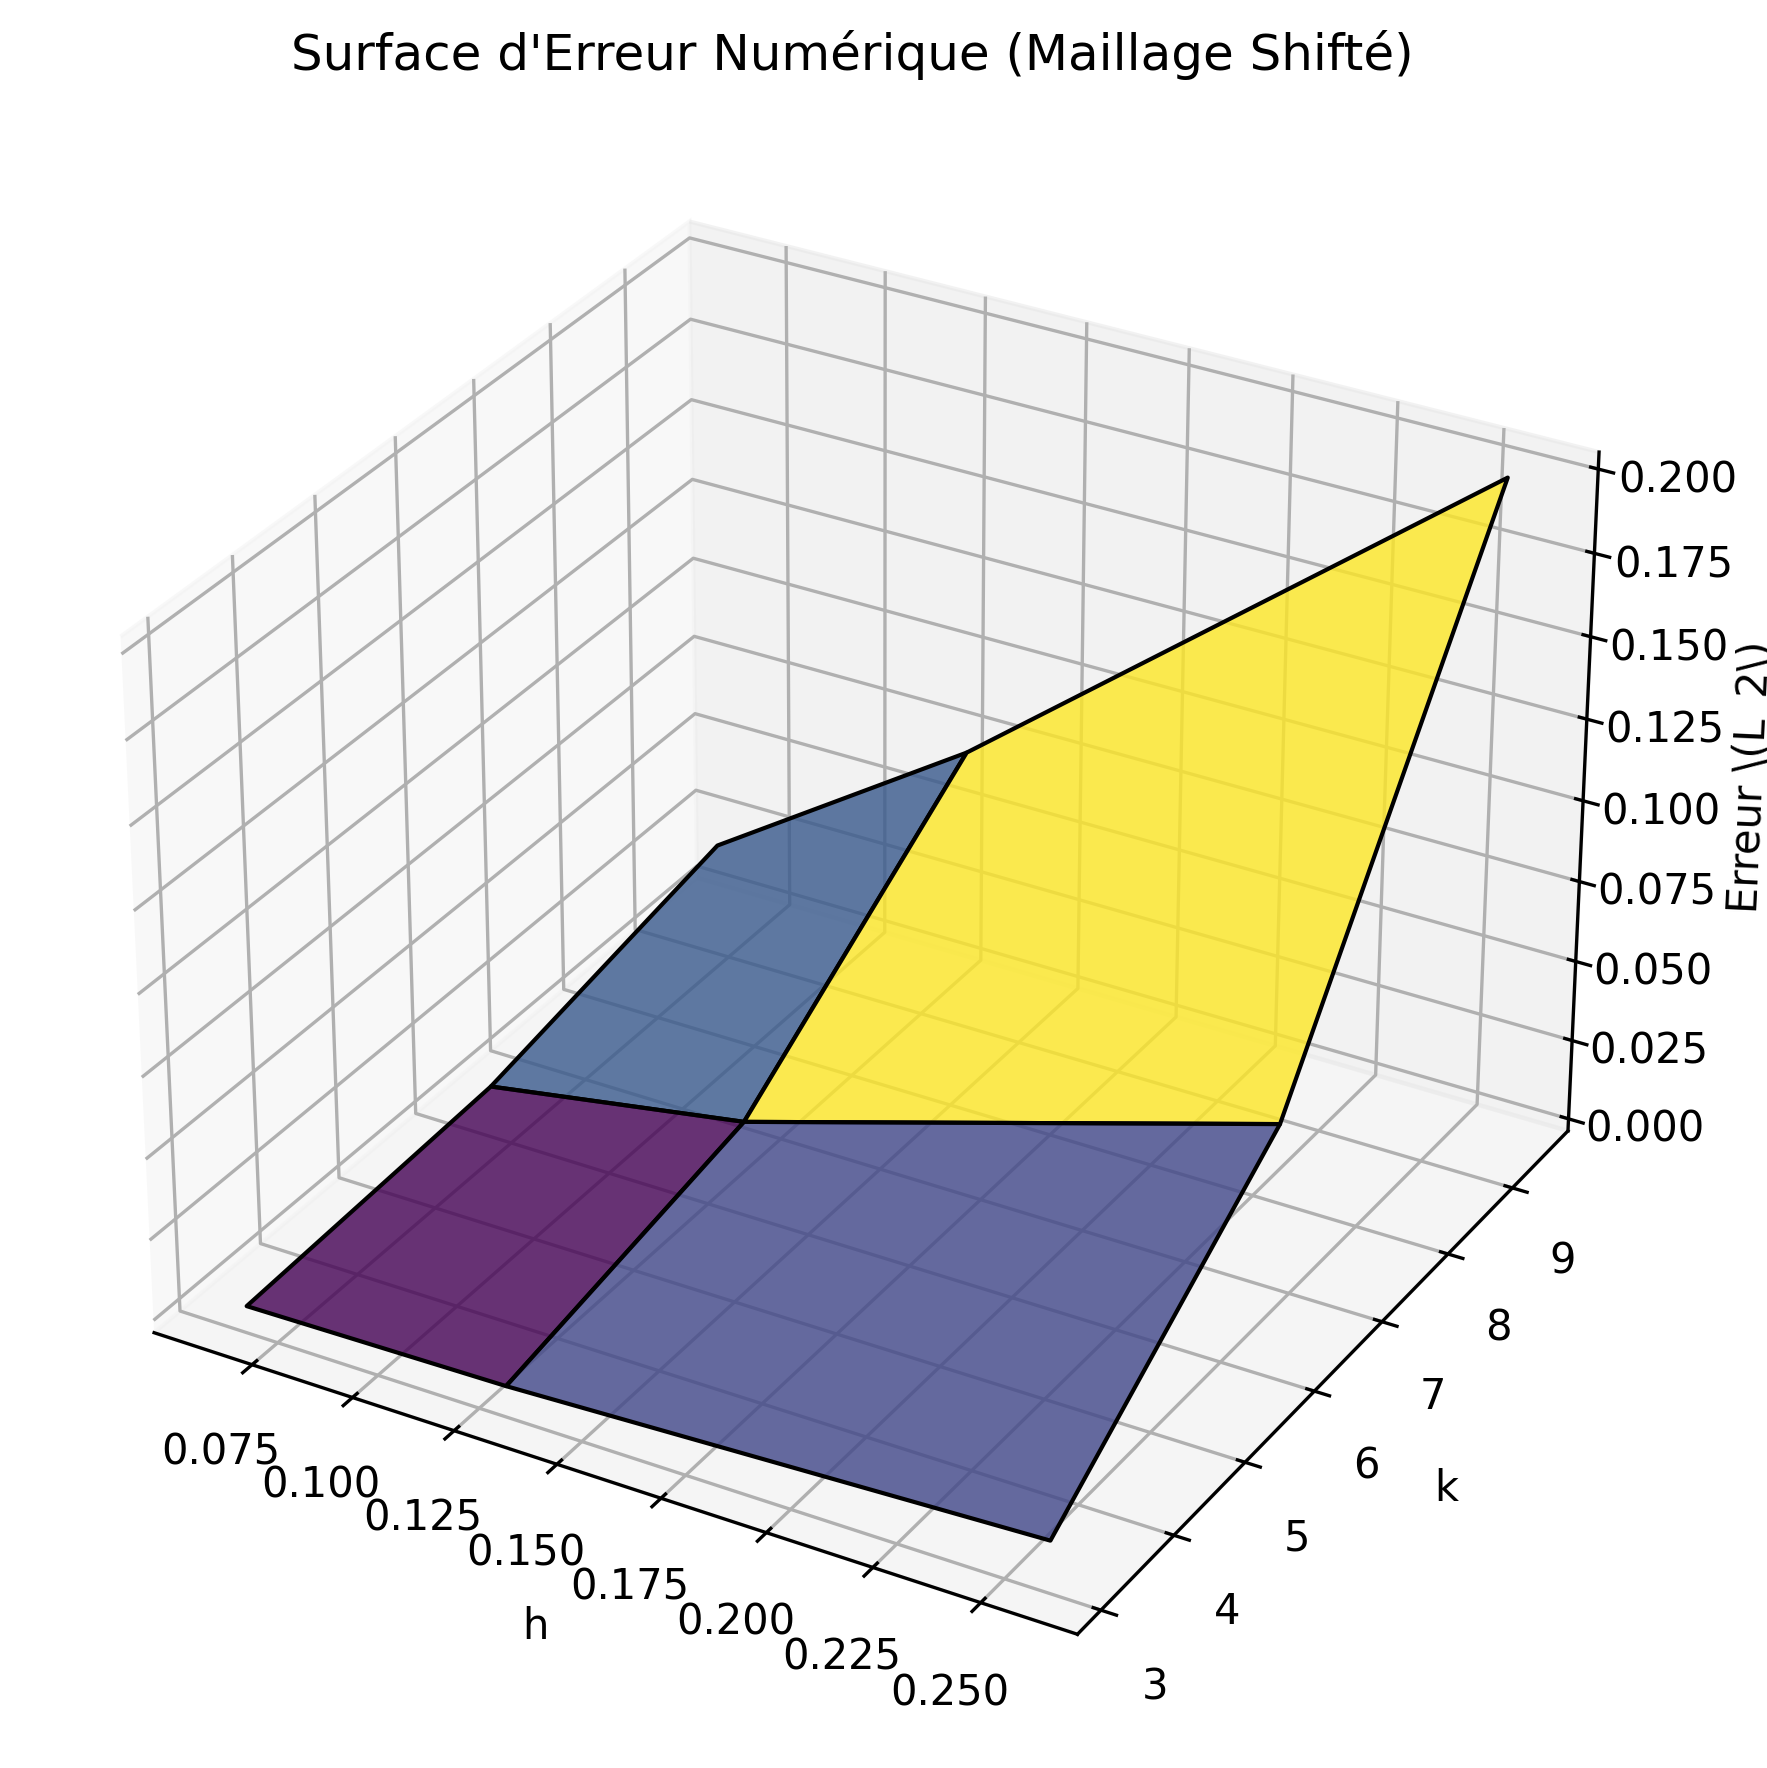
\includegraphics[width=0.55\textwidth]{figures/Figure11.png}
    \caption{Surface tridimensionnelle d'erreur (maillage shifté).}
    \label{fig:c11}
\end{figure}
La surface tridimensionnelle (Figure \ref{fig:c11}) confirme la structure globale de l'erreur sous contrainte géométrique.

\begin{figure}[H]
    \centering
    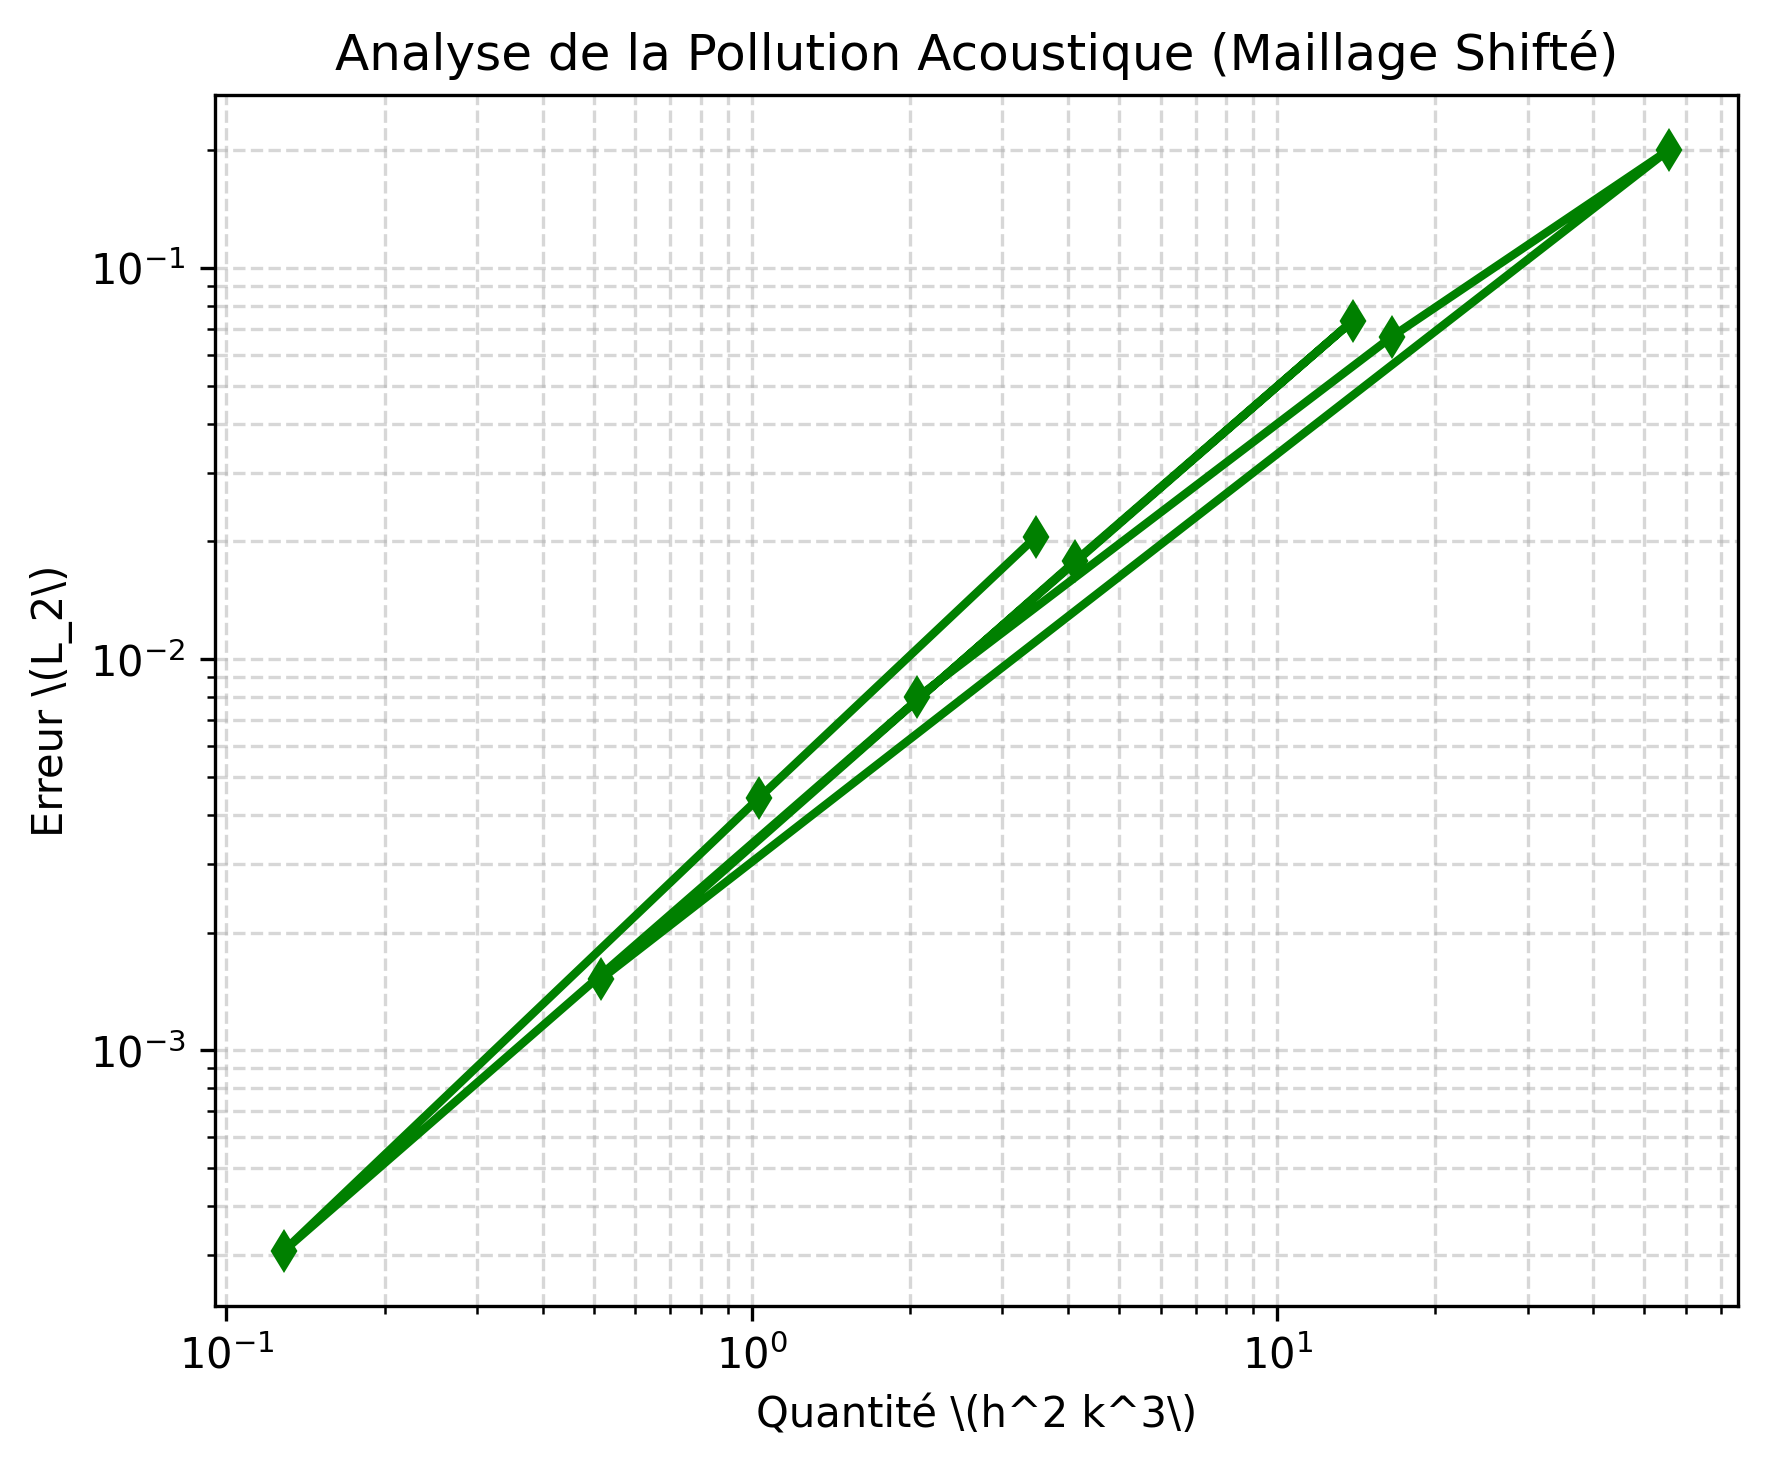
\includegraphics[width=0.55\textwidth]{figures/Figure12.png}
    \caption{Analyse de la pollution \(h^2 k^3\) (maillage shifté).}
    \label{fig:c12}
\end{figure}
La Figure \ref{fig:c12} atteste que le comportement de pollution reste le facteur limitant prépondérant à haute fréquence, indépendamment de la régularité initiale du maillage.

\section{Conclusion}
Ce travail de modélisation valide la robustesse de l'implémentation Python/SciPy. L'étude comparative entre maillage régulier (\(\alpha=1.93, \beta=3.80\)) et shifté (\(\alpha=2.35, \beta=3.53\)) démontre que si la convergence asymptotique est globalement préservée, la distorsion géométrique modifie l'amplitude des erreurs locales sans toutefois invalider la suprématie de la pollution acoustique à haute fréquence.

\end{document}